\documentclass[10pt,a4paper]{article}
\usepackage{amsmath}
\usepackage[
    colorlinks,
    citecolor=blue!70!black,
    linkcolor=blue!70!black,
    urlcolor=blue!70!black
]{hyperref}
\usepackage{tikz}
\usetikzlibrary{patterns}
\usepackage{xcolor}

\begin{document}

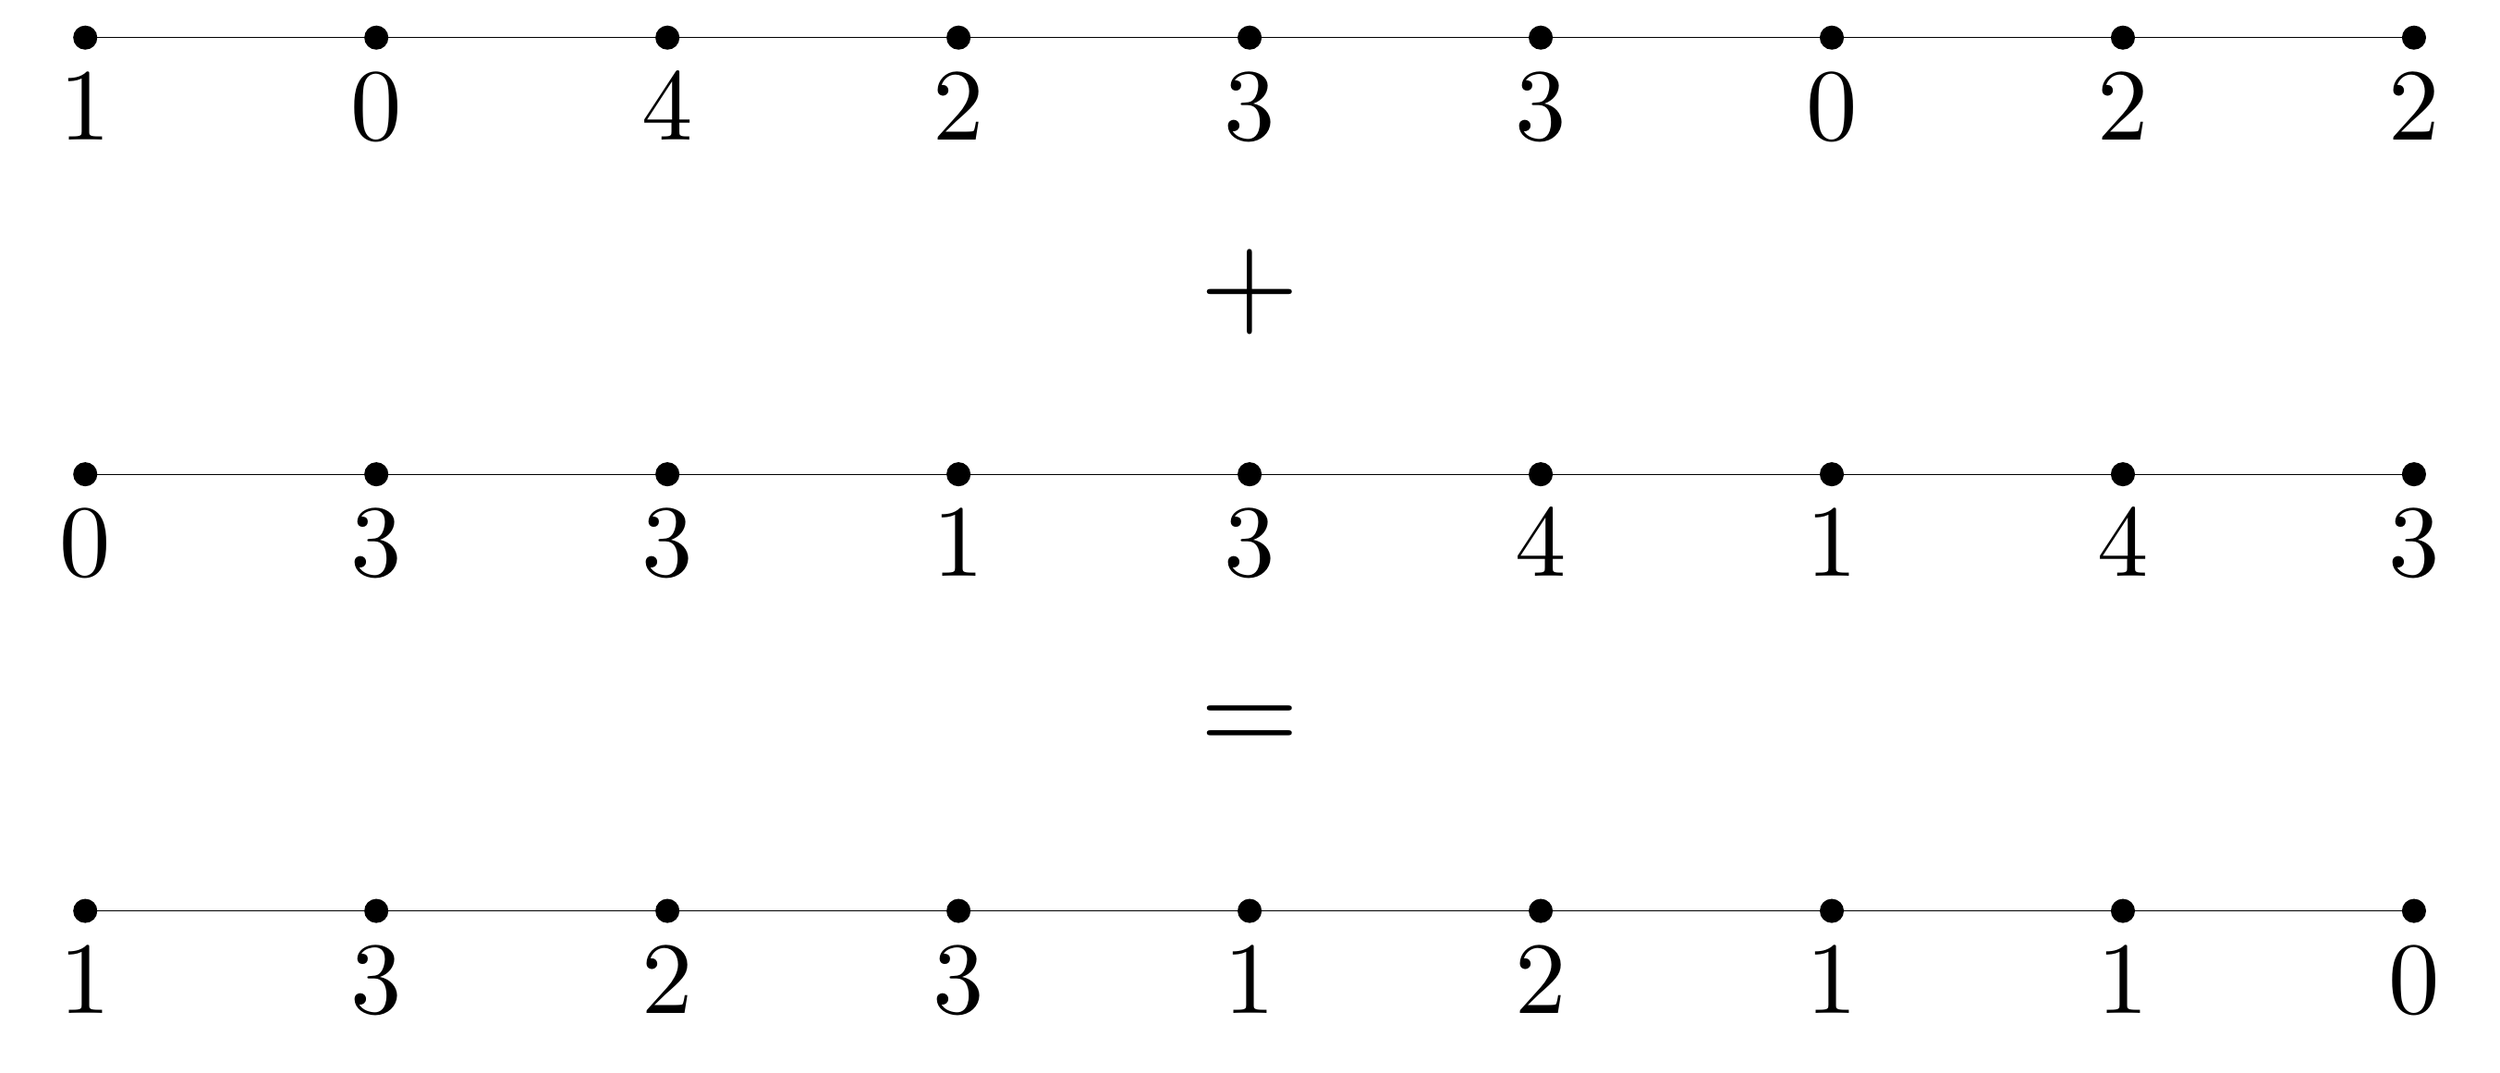
\begin{tikzpicture}
    	    \node[scale=5] at (16,8.5) {+};
    	    \node[scale=5] at (16,2.5) {=};
                \draw (0,12) -- (32,12);
        \node[scale=1] at (0,12) [circle,fill=black] {};
        \node[scale=4,below] at (0,12) {1};
        \node[scale=1] at (4,12) [circle,fill=black] {};
        \node[scale=4,below] at (4,12) {0};
        \node[scale=1] at (8,12) [circle,fill=black] {};
        \node[scale=4,below] at (8,12) {4};
        \node[scale=1] at (12,12) [circle,fill=black] {};
        \node[scale=4,below] at (12,12) {2};
        \node[scale=1] at (16,12) [circle,fill=black] {};
        \node[scale=4,below] at (16,12) {3};
        \node[scale=1] at (20,12) [circle,fill=black] {};
        \node[scale=4,below] at (20,12) {3};
        \node[scale=1] at (24,12) [circle,fill=black] {};
        \node[scale=4,below] at (24,12) {0};
        \node[scale=1] at (28,12) [circle,fill=black] {};
        \node[scale=4,below] at (28,12) {2};
        \node[scale=1] at (32,12) [circle,fill=black] {};
        \node[scale=4,below] at (32,12) {2};
        \draw (0,6) -- (32,6);
        \node[scale=1] at (0,6) [circle,fill=black] {};
        \node[scale=4,below] at (0,6) {0};
        \node[scale=1] at (4,6) [circle,fill=black] {};
        \node[scale=4,below] at (4,6) {3};
        \node[scale=1] at (8,6) [circle,fill=black] {};
        \node[scale=4,below] at (8,6) {3};
        \node[scale=1] at (12,6) [circle,fill=black] {};
        \node[scale=4,below] at (12,6) {1};
        \node[scale=1] at (16,6) [circle,fill=black] {};
        \node[scale=4,below] at (16,6) {3};
        \node[scale=1] at (20,6) [circle,fill=black] {};
        \node[scale=4,below] at (20,6) {4};
        \node[scale=1] at (24,6) [circle,fill=black] {};
        \node[scale=4,below] at (24,6) {1};
        \node[scale=1] at (28,6) [circle,fill=black] {};
        \node[scale=4,below] at (28,6) {4};
        \node[scale=1] at (32,6) [circle,fill=black] {};
        \node[scale=4,below] at (32,6) {3};
        \draw (0,0) -- (32,0);
        \node[scale=1] at (0,0) [circle,fill=black] {};
        \node[scale=4,below] at (0,0) {1};
        \node[scale=1] at (4,0) [circle,fill=black] {};
        \node[scale=4,below] at (4,0) {3};
        \node[scale=1] at (8,0) [circle,fill=black] {};
        \node[scale=4,below] at (8,0) {2};
        \node[scale=1] at (12,0) [circle,fill=black] {};
        \node[scale=4,below] at (12,0) {3};
        \node[scale=1] at (16,0) [circle,fill=black] {};
        \node[scale=4,below] at (16,0) {1};
        \node[scale=1] at (20,0) [circle,fill=black] {};
        \node[scale=4,below] at (20,0) {2};
        \node[scale=1] at (24,0) [circle,fill=black] {};
        \node[scale=4,below] at (24,0) {1};
        \node[scale=1] at (28,0) [circle,fill=black] {};
        \node[scale=4,below] at (28,0) {1};
        \node[scale=1] at (32,0) [circle,fill=black] {};
        \node[scale=4,below] at (32,0) {0};
     \end{tikzpicture}

\end{document}